% Options for packages loaded elsewhere
% Options for packages loaded elsewhere
\PassOptionsToPackage{unicode}{hyperref}
\PassOptionsToPackage{hyphens}{url}
\PassOptionsToPackage{dvipsnames,svgnames,x11names}{xcolor}
%
\documentclass[
  british,
  a4paper,
]{article}
\usepackage{xcolor}
\usepackage{amsmath,amssymb}
\setcounter{secnumdepth}{-\maxdimen} % remove section numbering
\usepackage{iftex}
\ifPDFTeX
  \usepackage[T1]{fontenc}
  \usepackage[utf8]{inputenc}
  \usepackage{textcomp} % provide euro and other symbols
\else % if luatex or xetex
  \usepackage{unicode-math} % this also loads fontspec
  \defaultfontfeatures{Scale=MatchLowercase}
  \defaultfontfeatures[\rmfamily]{Ligatures=TeX,Scale=1}
\fi
\usepackage{lmodern}
\ifPDFTeX\else
  % xetex/luatex font selection
\fi
% Use upquote if available, for straight quotes in verbatim environments
\IfFileExists{upquote.sty}{\usepackage{upquote}}{}
\IfFileExists{microtype.sty}{% use microtype if available
  \usepackage[]{microtype}
  \UseMicrotypeSet[protrusion]{basicmath} % disable protrusion for tt fonts
}{}
\makeatletter
\@ifundefined{KOMAClassName}{% if non-KOMA class
  \IfFileExists{parskip.sty}{%
    \usepackage{parskip}
  }{% else
    \setlength{\parindent}{0pt}
    \setlength{\parskip}{6pt plus 2pt minus 1pt}}
}{% if KOMA class
  \KOMAoptions{parskip=half}}
\makeatother
% Make \paragraph and \subparagraph free-standing
\makeatletter
\ifx\paragraph\undefined\else
  \let\oldparagraph\paragraph
  \renewcommand{\paragraph}{
    \@ifstar
      \xxxParagraphStar
      \xxxParagraphNoStar
  }
  \newcommand{\xxxParagraphStar}[1]{\oldparagraph*{#1}\mbox{}}
  \newcommand{\xxxParagraphNoStar}[1]{\oldparagraph{#1}\mbox{}}
\fi
\ifx\subparagraph\undefined\else
  \let\oldsubparagraph\subparagraph
  \renewcommand{\subparagraph}{
    \@ifstar
      \xxxSubParagraphStar
      \xxxSubParagraphNoStar
  }
  \newcommand{\xxxSubParagraphStar}[1]{\oldsubparagraph*{#1}\mbox{}}
  \newcommand{\xxxSubParagraphNoStar}[1]{\oldsubparagraph{#1}\mbox{}}
\fi
\makeatother


\usepackage{longtable,booktabs,array}
\newcounter{none} % for unnumbered tables
\usepackage{calc} % for calculating minipage widths
% Correct order of tables after \paragraph or \subparagraph
\usepackage{etoolbox}
\makeatletter
\patchcmd\longtable{\par}{\if@noskipsec\mbox{}\fi\par}{}{}
\makeatother
% Allow footnotes in longtable head/foot
\IfFileExists{footnotehyper.sty}{\usepackage{footnotehyper}}{\usepackage{footnote}}
\makesavenoteenv{longtable}
\usepackage{graphicx}
\makeatletter
\newsavebox\pandoc@box
\newcommand*\pandocbounded[1]{% scales image to fit in text height/width
  \sbox\pandoc@box{#1}%
  \Gscale@div\@tempa{\textheight}{\dimexpr\ht\pandoc@box+\dp\pandoc@box\relax}%
  \Gscale@div\@tempb{\linewidth}{\wd\pandoc@box}%
  \ifdim\@tempb\p@<\@tempa\p@\let\@tempa\@tempb\fi% select the smaller of both
  \ifdim\@tempa\p@<\p@\scalebox{\@tempa}{\usebox\pandoc@box}%
  \else\usebox{\pandoc@box}%
  \fi%
}
% Set default figure placement to htbp
\def\fps@figure{htbp}
\makeatother



\ifLuaTeX
\usepackage[bidi=basic,shorthands=off]{babel}
\else
\usepackage[bidi=default,shorthands=off]{babel}
\fi
\ifLuaTeX
  \usepackage{selnolig} % disable illegal ligatures
\fi


\setlength{\emergencystretch}{3em} % prevent overfull lines

\providecommand{\tightlist}{%
  \setlength{\itemsep}{0pt}\setlength{\parskip}{0pt}}



 


\makeatletter
\@ifpackageloaded{tcolorbox}{}{\usepackage[skins,breakable]{tcolorbox}}
\@ifpackageloaded{fontawesome5}{}{\usepackage{fontawesome5}}
\definecolor{quarto-callout-color}{HTML}{909090}
\definecolor{quarto-callout-note-color}{HTML}{0758E5}
\definecolor{quarto-callout-important-color}{HTML}{CC1914}
\definecolor{quarto-callout-warning-color}{HTML}{EB9113}
\definecolor{quarto-callout-tip-color}{HTML}{00A047}
\definecolor{quarto-callout-caution-color}{HTML}{FC5300}
\definecolor{quarto-callout-color-frame}{HTML}{acacac}
\definecolor{quarto-callout-note-color-frame}{HTML}{4582ec}
\definecolor{quarto-callout-important-color-frame}{HTML}{d9534f}
\definecolor{quarto-callout-warning-color-frame}{HTML}{f0ad4e}
\definecolor{quarto-callout-tip-color-frame}{HTML}{02b875}
\definecolor{quarto-callout-caution-color-frame}{HTML}{fd7e14}
\makeatother
\makeatletter
\@ifpackageloaded{caption}{}{\usepackage{caption}}
\AtBeginDocument{%
\ifdefined\contentsname
  \renewcommand*\contentsname{Table of contents}
\else
  \newcommand\contentsname{Table of contents}
\fi
\ifdefined\listfigurename
  \renewcommand*\listfigurename{List of Figures}
\else
  \newcommand\listfigurename{List of Figures}
\fi
\ifdefined\listtablename
  \renewcommand*\listtablename{List of Tables}
\else
  \newcommand\listtablename{List of Tables}
\fi
\ifdefined\figurename
  \renewcommand*\figurename{Figure}
\else
  \newcommand\figurename{Figure}
\fi
\ifdefined\tablename
  \renewcommand*\tablename{Table}
\else
  \newcommand\tablename{Table}
\fi
}
\@ifpackageloaded{float}{}{\usepackage{float}}
\floatstyle{ruled}
\@ifundefined{c@chapter}{\newfloat{codelisting}{h}{lop}}{\newfloat{codelisting}{h}{lop}[chapter]}
\floatname{codelisting}{Listing}
\newcommand*\listoflistings{\listof{codelisting}{List of Listings}}
\makeatother
\makeatletter
\makeatother
\makeatletter
\@ifpackageloaded{caption}{}{\usepackage{caption}}
\@ifpackageloaded{subcaption}{}{\usepackage{subcaption}}
\makeatother
\usepackage{bookmark}
\IfFileExists{xurl.sty}{\usepackage{xurl}}{} % add URL line breaks if available
\urlstyle{same}
% fallback for those not using the hyperref driver hyperxmp:
\makeatletter
\@ifundefined{xmpquote}{\newcommand{\xmpquote}[1]{#1}}{}
\makeatother
\hypersetup{
  pdftitle={Demographics and growth in emerging markets},
  pdfauthor={Carlos Galindo},
  pdflang={en-GB},
  colorlinks=true,
  linkcolor={blue},
  filecolor={Maroon},
  citecolor={Blue},
  urlcolor={Blue},
  pdfcreator={LaTeX via pandoc}}


\title{Demographics and growth in emerging markets}
\usepackage{etoolbox}
\makeatletter
\providecommand{\subtitle}[1]{% add subtitle to \maketitle
  \apptocmd{\@title}{\par {\large #1 \par}}{}{}
}
\makeatother
\subtitle{How demographics and social conditions line up with projected
long-run growth across eighteen emerging economies}
\author{Carlos Galindo}
\date{}
\begin{document}
\maketitle


\begin{tcolorbox}[enhanced jigsaw, arc=.35mm, bottomrule=.15mm, breakable, colback=white, colframe=quarto-callout-note-color-frame, left=2mm, leftrule=.75mm, opacityback=0, rightrule=.15mm, toprule=.15mm]

\vspace{-3mm}\textbf{At a glance}\vspace{3mm}

\begin{itemize}
\tightlist
\item
  \textbf{Question.} How far do a country's demographic trajectory and
  its social conditions together explain how fast an emerging economy
  can grow over the next two decades?
\item
  \textbf{Approach.} Pair published population projections with public
  social indicators for 18 economies, reduce each block to a single
  factor, and compare both factors with projected potential growth.
\item
  \textbf{Finding.} Estimated on one frozen dataset, working-age growth
  (+0.25) and inequality (−0.22) point the expected way but cannot be
  told apart from zero in 18 economies. Only urbanisation has a link
  whose 95\% interval excludes zero, and it is negative, a level effect.
  A demographic and a social factor each line up with growth, in
  opposite directions, and cancel in an equal-weight composite.
\item
  \textbf{Why it matters.} It tests the ``demographic dividend'' story
  against the projections themselves, and checks each early correlation
  against a frozen re-run, so that only relationships that hold carry
  the conclusions.
\end{itemize}

\end{tcolorbox}

\subsection{The question}\label{the-question}

Demographics is the slow variable in macroeconomics. Births, deaths and
migration set the size of the workforce a generation ahead, and they are
known with far more confidence than almost anything else in a long-run
forecast. The popular story is that a young, growing population is a
growth engine and an ageing one is a drag.

That story is incomplete in a way that matters to anyone allocating
attention or capital across emerging markets. A large cohort of
working-age people is a potential, not an outcome. It becomes growth
only when those people are educated, healthy, employed and able to move
up, and when savings and investment follow. This project asked a simple
question of that framework: across a broad group of emerging economies,
how much of projected growth lines up with demography, and how much with
the social conditions that decide whether demography pays?

The work was a research note and a presentation, written and delivered
in under a week in spring 2025. It was built to be read by
decision-makers, so it favours a clear structure and a short list of
takeaways over econometric detail.

\subsection{Approach}\label{approach}

\textbf{Coverage.} The sample covers 18 emerging economies across Latin
America, emerging Asia, Central and Eastern Europe, the Middle East and
Africa. For each one the project assembled projected annual growth of
total and economically active population over 2024--2044, the year in
which the working-age population peaks, the year in which the dependency
ratio crosses one half, and projected potential output growth over the
same horizon taken from published external work. A second block of
public indicators described social conditions: literacy, urbanisation,
income inequality, life expectancy, connectivity, access to electricity,
and spending on education and health.

\textbf{Framework.} The note starts from the demographic dividend: a
falling dependency ratio opens a window in which savings, investment and
productivity can rise, provided human capital and social mobility keep
up. It also treats the mirror image, demographic drag, when the
workforce shrinks and the dependency burden climbs.

\textbf{Factors.} To avoid choosing among dozens of overlapping
indicators, each block was standardised and reduced to its first
principal component. The demographic factor was built from six
population variables and the social fabric factor from twelve variables
on education, infrastructure and well-being. A composite score averaged
the two with equal weights. Each country's score can be decomposed into
the contribution of every underlying variable, which makes the ranking
explainable in a meeting rather than a black box.

\textbf{Reading the relationships.} Factors and individual indicators
were set against projected potential growth with correlations, simple
regressions and a quadrant map that sorts countries by strength of
demography and strength of social fabric. A cluster analysis grouped
economies with similar profiles. A comparison across several published
long-run growth scenarios gave a sense of how wide the disagreement over
each country's trajectory is.

\subsection{What the work shows}\label{what-the-work-shows}

\textbf{Demography lines up with growth, weakly.} On the frozen table of
18 economies, growth of the economically active population and projected
potential growth have a correlation of +0.25, with a 95\% interval from
−0.25 to +0.64. The sign is the one the dividend story predicts, but 18
observations cannot separate it from zero. Total population growth adds
nothing beyond it: in the source table the two series differ by a
constant in every economy.

\begin{figure}

\centering{

\pandocbounded{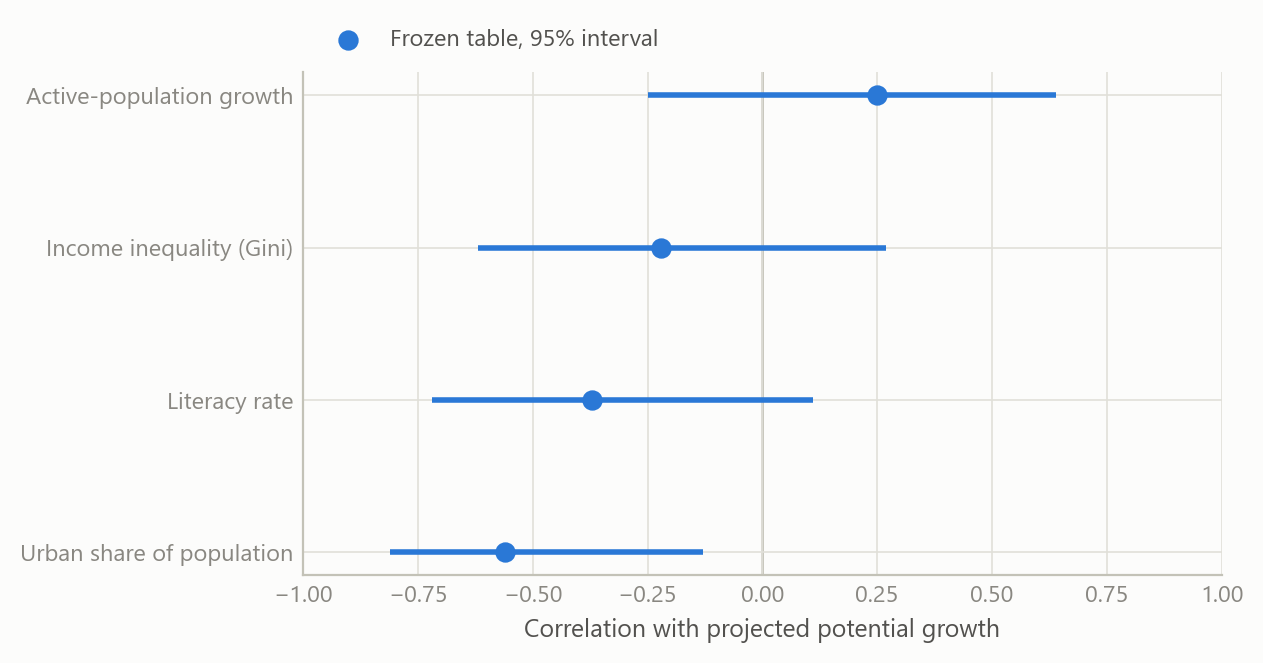
\includegraphics[keepaspectratio]{index_files/figure-latex/fig-demography-growth-output-1.png}}

}

\caption{\label{fig-demography-growth}Correlation of each indicator with
projected potential growth, 18 emerging economies, 2024-2044. Dots:
frozen final table, with 95\% intervals. Source: the project's final
18-economy table (published population projections, long-run growth
scenarios and development indicators); the author's calculations.}

\end{figure}%

\textbf{Inequality: the sign survives, the strength does not.} The
spring summary put the inequality-growth correlation at about −0.74, the
strongest of the social links. The frozen table gives −0.22, with an
interval from −0.62 to +0.27, and the rank correlation is only −0.08.
The earlier figure most likely came from a wider early sample that
included several Gulf economies and Egypt, which the final table does
not contain. The one link whose interval excludes zero is urbanisation,
at −0.56 (−0.81 to −0.13), with literacy at −0.37 close behind. These
negative signs look perverse until one notices who is in the sample:
economies that are already highly urbanised and literate are the mature
ones, with lower growth ceilings. These are level effects, not evidence
that schooling or cities hurt growth. The note says so plainly, because
a naive reading would recommend the opposite of what the development
literature shows. Adding the United States to the sample moves none of
the four correlations by more than 0.03.

\textbf{The standout cases are the instructive ones.}

\begin{itemize}
\tightlist
\item
  India combines a growing workforce, with its working-age population
  peaking around 2032, with the highest projected potential growth of
  the group, despite the weakest social scorecard on literacy and
  urbanisation. Its case rests on scale and on the scope for upward
  mobility if policy delivers.
\item
  South Africa has a similarly favourable demographic profile but the
  lowest projected potential growth of the group. Inequality and weak
  human capital are the standard explanation, and it is the clearest
  example of a dividend that goes uncollected.
\item
  Korea and Taiwan show the opposite: shrinking workforces, high
  literacy and low inequality, and growth sustained by productivity.
\end{itemize}

\textbf{Two factors, four quadrants.} Plotting the demographic factor
against the social fabric factor sorts the economies into four groups:
strong on both, strong demography with weak social fabric, the reverse,
and weak on both. The factors summarise their blocks unevenly: the first
demographic component captures 0.63 of the variance of its six
variables, the social component 0.44 of its twelve. On the frozen table
the demographic factor correlates at +0.64 with projected growth
(R-squared 0.40), but its loadings are dominated by population size, so
it mostly says that India and China are both large and fast-growing. The
social factor correlates at −0.52 (R-squared 0.27): the mature,
well-served economies are projected to grow more slowly, which is
convergence rather than a social drag. Because the two point in opposite
directions, the equal-weight composite explains almost nothing
(R-squared 0.001).

\begin{figure}

\centering{

\pandocbounded{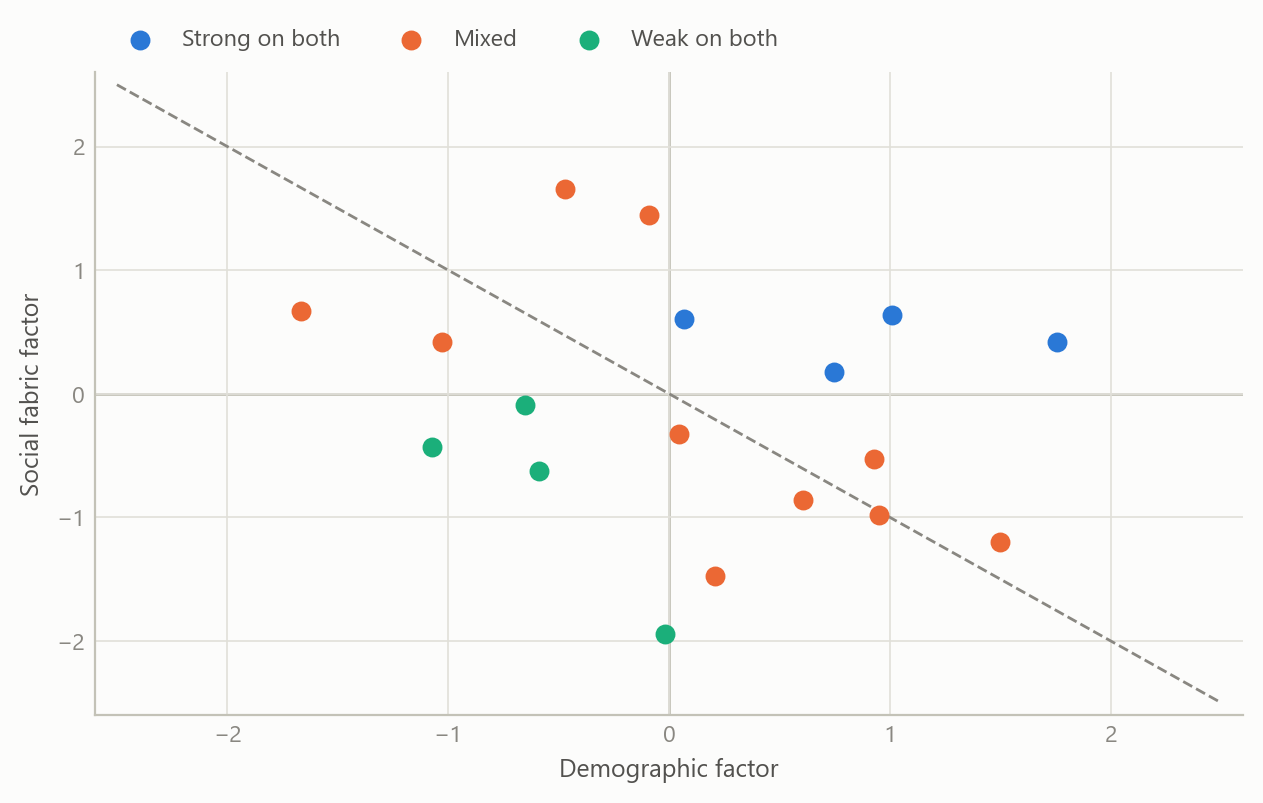
\includegraphics[keepaspectratio]{index_files/figure-latex/fig-quadrants-output-1.png}}

}

\caption{\label{fig-quadrants}Demographic factor against social fabric
factor for 18 economies, grouped by quadrant, with the equal-weight
composite as the diagonal (simulated data).}

\end{figure}%

\textbf{The timing matters as much as the level.} The most useful single
variable for a decision-maker is not the growth rate of the population
but when the dependency ratio crosses one half, and when the workforce
peaks. Some economies are decades from that threshold, others have
already passed it. The stylised paths below show three types of profile.

\begin{figure}

\centering{

\pandocbounded{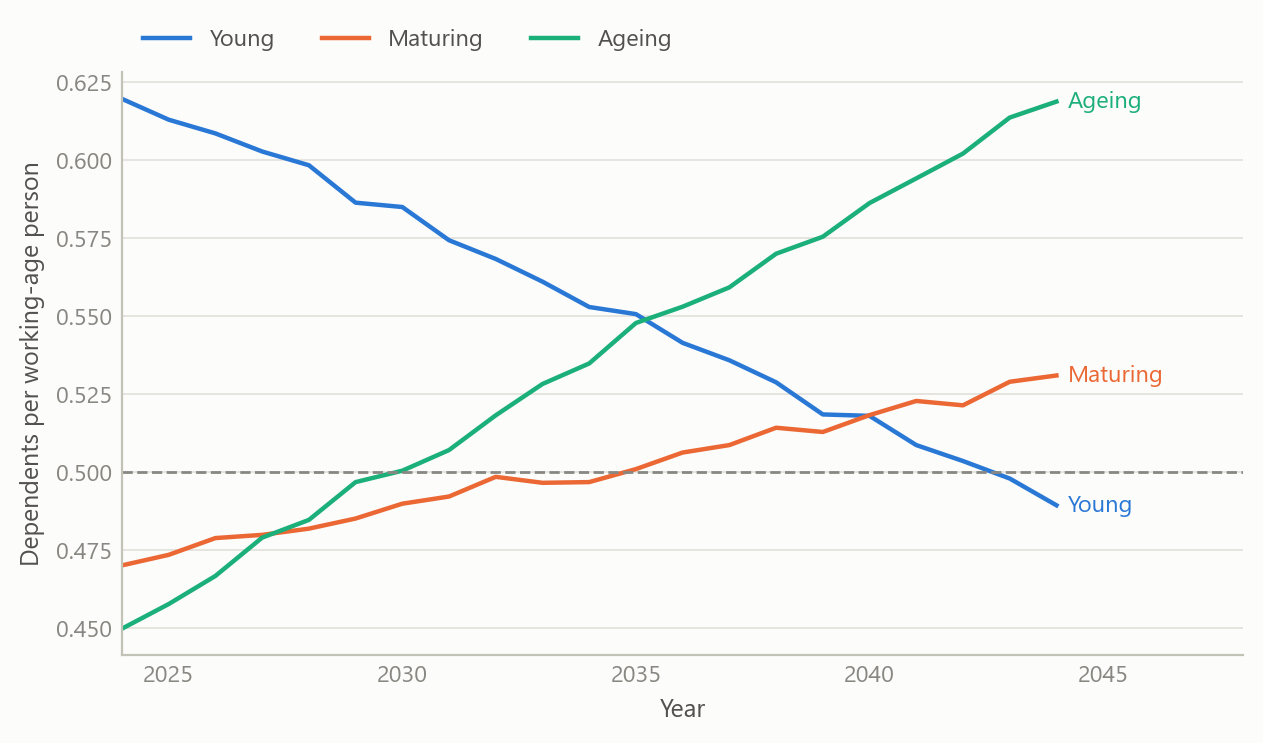
\includegraphics[keepaspectratio]{index_files/figure-latex/fig-dependency-output-1.png}}

}

\caption{\label{fig-dependency}Stylised dependency-ratio paths,
2024-2044, for a young, a maturing and an ageing economy; the dashed
line is the one-half threshold (simulated data).}

\end{figure}%

\subsection{Insights}\label{insights}

\begin{enumerate}
\def\labelenumi{\arabic{enumi}.}
\tightlist
\item
  \textbf{Eighteen economies cannot confirm a dividend.} Working-age
  growth and inequality carry the expected signs, but neither interval
  excludes zero. The same working-age growth appears alongside very
  different projected growth, and India and South Africa sit at opposite
  ends of the group with similar demographic profiles.
\item
  \textbf{A composite can hide two signals.} The demographic and social
  factors each line up with projected growth, in opposite directions,
  and an equal-weight average cancels them. Look at the components
  before trusting an index.
\item
  \textbf{Productivity can offset shrinking numbers.} The high-literacy,
  low-inequality economies with falling workforces still show
  respectable projected growth, which says that the weight falls on
  output per worker.
\item
  \textbf{Timing beats averages.} The year a workforce peaks and the
  year the dependency ratio crosses one half say more about the
  investment horizon than a twenty-year average growth rate.
\item
  \textbf{Level effects mislead.} Negative correlations for literacy and
  urbanisation reflect mature economies with lower growth ceilings, not
  a harm from education.
\item
  \textbf{Disagreement among scenarios is information.} Long-run growth
  scenarios from different institutions can differ by several percentage
  points for the same country, so a single projection should not be
  treated as a fact.
\end{enumerate}

\subsection{Scope and next steps}\label{scope-and-next-steps}

The study is built to test the demographic-dividend argument against
long-run growth projections across a cross-section of economies, on one
frozen table, so that every quoted value traces to a single source.
Because the projections embed demographic assumptions of their own, it
reads how forecasts line up with fundamentals.

The natural extensions are four. First, a demographic factor built from
the speed and timing of population change rather than its size. Second,
dependency-ratio timing as an explicit regressor, and a measure of
productivity growth. Third, realised growth outcomes in place of
projections, to move from how forecasts line up with fundamentals to
what fundamentals cause. Fourth, a wider sample of economies, to test
whether the working-age and inequality effects hold in a larger
cross-section.

\subsection{About the evidence}\label{about-the-evidence}

The note and presentation were produced in spring 2025, using published
population projections, published long-run growth scenarios and public
development indicators for 18 emerging economies. Correlations,
intervals and explained variance in the text are estimated on the
project's frozen final table of 18 economies, with 95\% intervals from
the Fisher transformation. The correlation chart shows these derived
statistics, not the underlying third-party projections. The quadrant
chart and the dependency-ratio paths are simulated to share the
structure of the analysis and are not the project's results.

Figures and tables marked \emph{simulated} are generated from simulated
data built to share the structure of the analysis (its variables,
horizons and frequencies). They show how each method works and what its
output looks like. Results stated in the text, and figures that give a
source, are the project's own. Methods are described at the level of a
methods section. Code and data pipelines are not reproduced here.




\end{document}
